\documentclass[border=8pt]{standalone}
\usepackage{pgfplots}
\pgfplotsset{compat=1.18}
\begin{document}
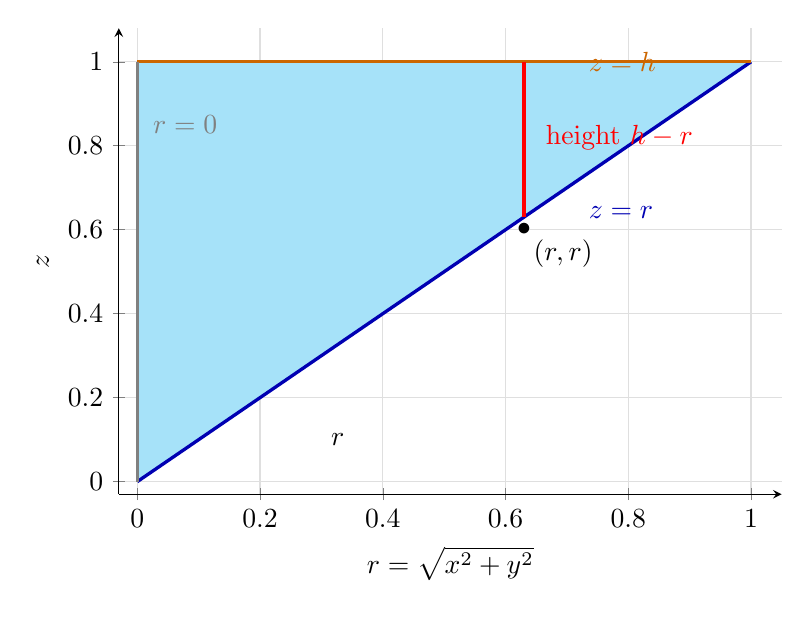
\begin{tikzpicture}
\begin{axis}[
    axis lines=left,
    xlabel={$r=\sqrt{x^2+y^2}$}, ylabel={$z$},
    xmin=-0.03, xmax=1.05, ymin=-0.03, ymax=1.08,
    width=10cm, height=7.5cm,
    ytick={0,0.2,...,1}, xtick={0,0.2,...,1},
    grid=both, grid style={gray!25},
]
% shaded region 0 <= r <= z <= h
\addplot[fill=cyan!35, draw=none] coordinates {(0,0) (1,1) (0,1)} \closedcycle;
% boundaries
\addplot[very thick, blue!70!black, domain=0:1] {x};
\addplot[very thick, orange!80!black, domain=0:1] {1};
\addplot[very thick, gray, domain=0:1] coordinates {(0,0) (0,1)};
% sample strip
\addplot[very thick, red] coordinates {(0.63,0.63) (0.63,1)};
% annotations
\node[red, right] at (axis cs:0.65,0.82) {height $h-r$};
\node[black, right] at (axis cs:0.30,0.10) {$r$};
\node[blue!70!black, right] at (axis cs:0.72,0.64) {$z=r$};
\node[orange!80!black, right] at (axis cs:0.72,1.0) {$z=h$};
\node[gray, right] at (axis cs:0.01,0.85) {$r=0$};
\node at (axis cs:0.63,0.60) {$\bullet$};
\node[below right] at (axis cs:0.63,0.60) {$(r,r)$};
\legend{}
\end{axis}
\end{tikzpicture}
\end{document}
